
% http://patorjk.com/software/taag/#p=display&f=Colossal&t=ABOUT
\documentclass[runningheads,a4paper,oribibl]{llncs}
%\setcounter{secnumdepth}{4}

\usepackage[T1]{fontenc}

\usepackage[utf8]{inputenc}
%\usepackage[latin1]{inputenc}
\usepackage{textcomp}

\usepackage{graphicx}    
\usepackage{url}
\usepackage{pdfpages}  


%My packages
\usepackage{array}





       

\begin{document}

\pagestyle{headings}

\mainmatter

\title{Exploring the differences in performance between gamers and non-gamers when completing tasks viewed from a third-person perspective}


\titlerunning{Third-Person Performance Differences Between Gamers and Non-gamers}

\author{Arvid Bräne}

\institute{
	Department of Computing Science \\
	Umeå University, Sweden. \\
	Email: \email{arvidbrane@gmail.com} \\
   Website: \url{http://www.arvidbrane.se}
}

\maketitle


\begin{abstract}
The concept of third-person perspective in gaming has been around since the start of graphics in video games. This study aims to investigate if there is a measurable difference in performance between gamers and non-gamers when they complete the same tasks from a third-person perspective. Experiments were made using a back-mounted camera rig and pair of video goggles. Results, generated from a small amount of participants, suggest that there is no significant difference in performance between the two groups when adjusting to a third-person view.
	

%What to take out from this study.

\end{abstract}









% 8888888 888b    888 88888888888 8888888b.   .d88888b.  
%   888   8888b   888     888     888   Y88b d88P" "Y88b 
%   888   88888b  888     888     888    888 888     888 
%   888   888Y88b 888     888     888   d88P 888     888 
%   888   888 Y88b888     888     8888888P"  888     888 
%   888   888  Y88888     888     888 T88b   888     888 
%   888   888   Y8888     888     888  T88b  Y88b. .d88P 
% 8888888 888    Y888     888     888   T88b  "Y88888P"  


\section{Introduction}
% Description of what third-person view is


There is a constantly ongoing debate on whether playing video games produce negative side-effects or not~\cite{tear2014video}. Some studies suggest links between violent video games and increases aggressive behavior, decreases in helping behavior~\cite{anderson2004update} and decreased prosocial behavior~\cite{anderson2001effects}. Earlier findings indicate that committing ``immoral'' virtual behaviors in a video game can lead to increased moral sensitivity of the player~\cite{grizzard2014being} and that playing video games do not have any effect on depression, hostility, or visuospatial cognition~\cite{valadez2012just}. There are even results in experiments that suggest violent games reduce depression and hostile feelings in players through mood management~\cite{ferguson2015hitman}. There is also research hinting that video games can result in positive side-effects such as improved cognitive control, emotional regulation, spatial resolution of vision, hand-eye motor coordination, and contrast sensitivity~\cite{gong2015enhanced}. Other results point towards an improved decision making (probabilistic inference) without loss of measurable accuracy~\cite{green2010improved}.

This study aims to investigate if there is a measurable difference in performance, such as number of errors made and time consumption, between people who have played video games (gamers) and people who have not (non-gamers) when they are prompted to complete specific tasks viewed from third-person perspective\footnote{A perspective were the view is at a fixed distance behind and slightly above the user, often used in video games.} (see Figure \ref{fig:GTAIV}). Similar studies have been conducted, both survey based questioners~\cite{schmierbach2011exploring} and game-related experiments using augmented reality~\cite{nakamura20103pi}, but certain aspects about performance differences in tasks that heavily depend on orientation, navigation and balance remain unaddressed. This study was completed using a custom-made rig in order to simulate the experience of a life viewed from a third-person perspective.



\subsection{Earlier Work}
Studies in literature have previously shown that most readers do not have any recognition about whether a book they have read was written in first- or third-person~\cite{hagg2012nya} due to humans capability of ``translating'' and adapting from one pronoun to another. Kohler's experiments with inverted vision goggles showed subjects walking and riding bicycles while seeing upside-down~\cite{kohler1962goggles}, pointing towards even greater ability for the brain to adapt. This could suggest that users might be able to adapt to seeing themselves from third-person perspective in a relatively short time, something suggested by prior studies~\cite{nakamura20103pi}.

Experiments measuring navigation and movement performance~\cite{ruddle2013learning}, similar to our experiments, have also been conducted. These were performed in virtual reality (VR) using different interfaces (joystick-only, linear and omni- directional treadmills, and actual walking) to control their navigation in the VR world. Further studies suggest that walking interfaces are to be preferred when navigating three-dimensional virtual environments~\cite{ruddle2009benefits}.






















% 888b     d888 8888888888 88888888888 888    888  .d88888b.  8888888b.  
% 8888b   d8888 888            888     888    888 d88P" "Y88b 888  "Y88b 
% 88888b.d88888 888            888     888    888 888     888 888    888 
% 888Y88888P888 8888888        888     8888888888 888     888 888    888 
% 888 Y888P 888 888            888     888    888 888     888 888    888 
% 888  Y8P  888 888            888     888    888 888     888 888    888 
% 888   "   888 888            888     888    888 Y88b. .d88P 888  .d88P 
% 888       888 8888888888     888     888    888  "Y88888P"  8888888P"  

\section{Material \& Method}
Studies prior to this one have been done on the differences between gamers and non-gamers, such as~\cite{schmierbach2011exploring} and~\cite{gong2015enhanced}, but only a minority using hardware to simulate the out-of-body third-person view experienced in games (see Figure \ref{fig:GTAIV}) in real life. Our method of choice was to construct a custom designed rig where subjects saw themselves in real-time from a third-person perspective. In order to see the differences between the groups they had to complete the same three tasks in three different perspectives. After the subjects finished their participation, they were prompted to fill in a form regarding the experience and their prior experience with video games. The two groups, consisting of 13 subjects (undergraduate volunteers, 12 male subjects and two female, in ages ranging from 23 to 28), were benchmarked against each other to see which performed better. Originally there were 14 subjects in the study, however one participant could not complete the whole experiment due to the subjects poor eyesight when not wearing his glasses. This subject was therefore excluded from the study after the first task and not included in the results.




\begin{figure}
   \centering
   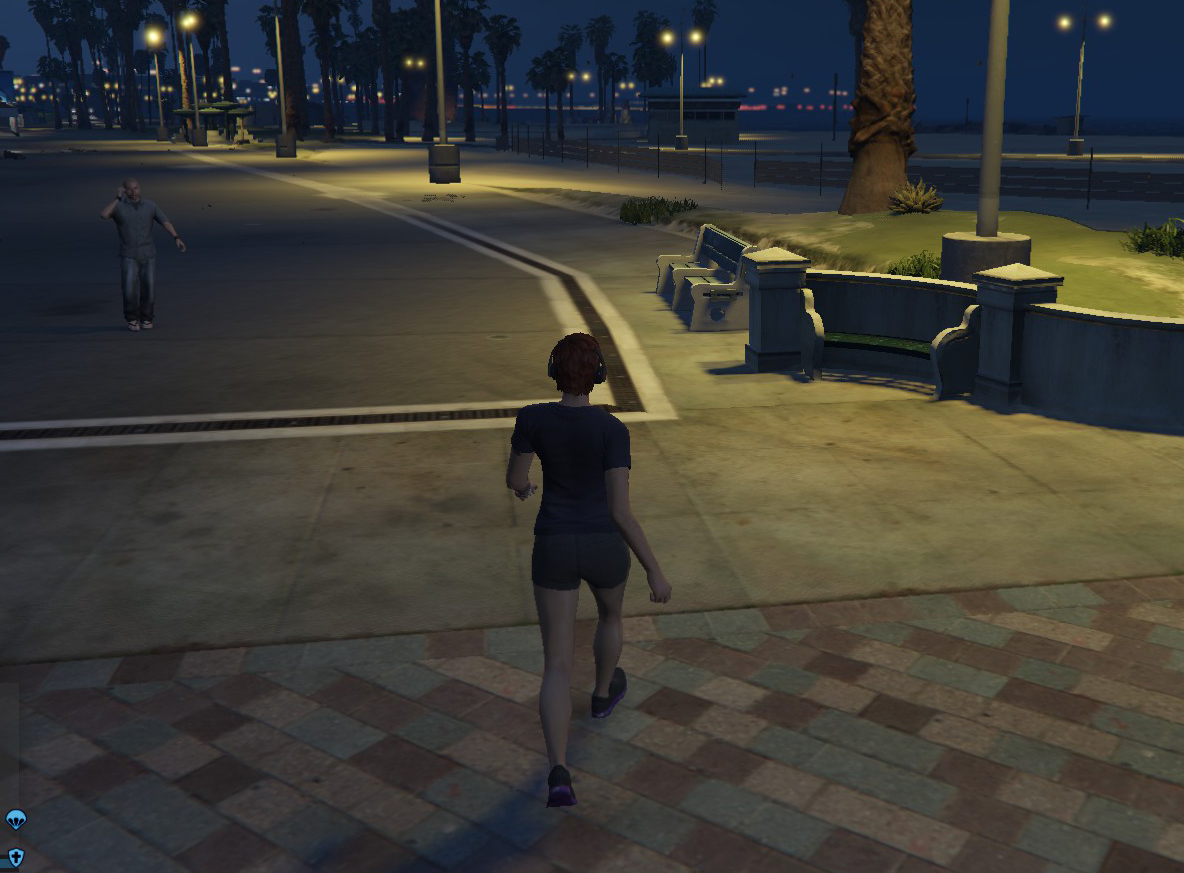
\includegraphics[width=0.8\textwidth]{ExternalMaterial/GTA}
   \caption{A typical third-person perspective from the game \emph{Grand Theft Auto: V}. The point of view is shifted from the typical position (the character's eyes) to behind and above the subject resulting in a wider and unreal field of view. \label{fig:GTAIV}}
\end{figure}



\subsection{Rig Design}
In order to fully simulate a game-like, out-of-body experience and a third-person perspective (see Figure \ref{fig:GTAIV}), without leaving the participants nauseated\footnote{Early test showed that participants felt sea-sick due to unwanted camera movement created by an unstable test-rig.} the rig had to be as rigid as possible. The main parts in the rig were:
\begin{description}
   \item[Back \&\ Camera Mount] A solid mounting foundation was constructed out of light weight and stiff materials such as carbon fiber, ABS and Polymorph\footnote{More info can be found at http://www.polymorphplastic.co.uk/} plastic. As a base a snowboard back protector was used in order to connect a carbon fiber rod to the subjects back. Some 3D-printed parts were used to fasten the third-person camera to the rod.

   \item[Third-Person Video Camera] The video camera used for the third-person view, constantly generating a live video stream, was mounted on a rod circa one meter and approximately 45 degrees above/behind the participants head and tilted circa 30 degrees downwards in order to frame the video correctly. Since a large field of view\footnote{The restriction in the visible view} and a compact- and lightweight design were the most important requirements for selecting the video camera, a \emph{GoPro Hero 3: Black Edition}\footnote{More info can be found at https://goo.gl/dLW5uz} was chosen, weighing 163 grams and a diagonal field of view of 149 degrees. The camera was connected to the participants video goggles using a three meter long cable.
   % with a diagonal field of view of approximately 30 degrees
   \item[Video Goggles \&\ First-Person Video Camera] To cover the subjects eyes and view the video stream a pair of video goggles were used. These goggles, a pair of \emph{SkyZone SKY-01 V2}\footnote{More info can be found at http://www.foxtechfpv.com/skyzone-fpv-gogglesmatte-blackpreorder-p-1218.html}, have a built in screen and an onboard camera with a diagonal field of view at 120 degrees. This camera was used for the second configuration for each task (described in Section~\ref{subsubsec:Configurations}) to simulate first-person perspective.
\end{description}
The design was inspired by the rig used in \emph{Quantifying effects of exposure to the third and first-person perspectives in virtual-reality-based training}~\cite{salamin2010quantifying} (but with more up-to-date hardware) and is illustrated in Figure \ref{fig:RigDesign}. An approximation (the top and bottom of the image is cut of due to the camera not being able to capture non-wide screen video\footnote{During the experiment the user was able to see approximately 30 cm behind their feet.}) of what the subjects saw is demonstrated in Figure \ref{fig:3Pview}.



\begin{figure}
   \centering
   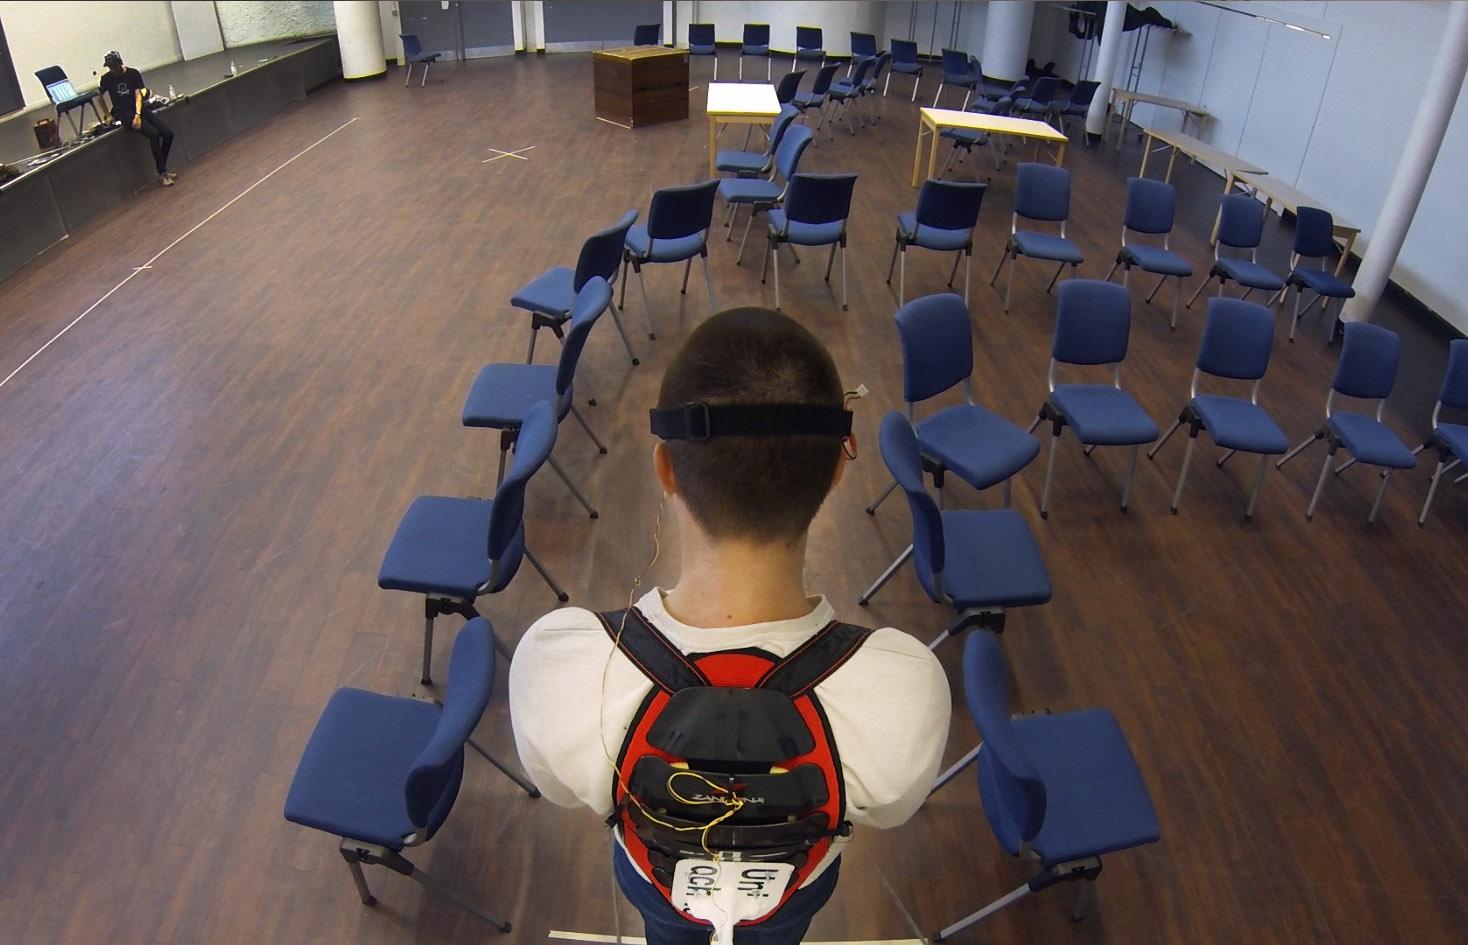
\includegraphics[width=\textwidth]{ExternalMaterial/3Pview}

   \caption{An approximate (the top and bottom of the image is cut of due to the camera not being able to capture non-wide screen video) view of what the participant saw in third-person configuration during the experiments. \label{fig:3Pview}}
\end{figure}



\begin{figure}
   \centering
   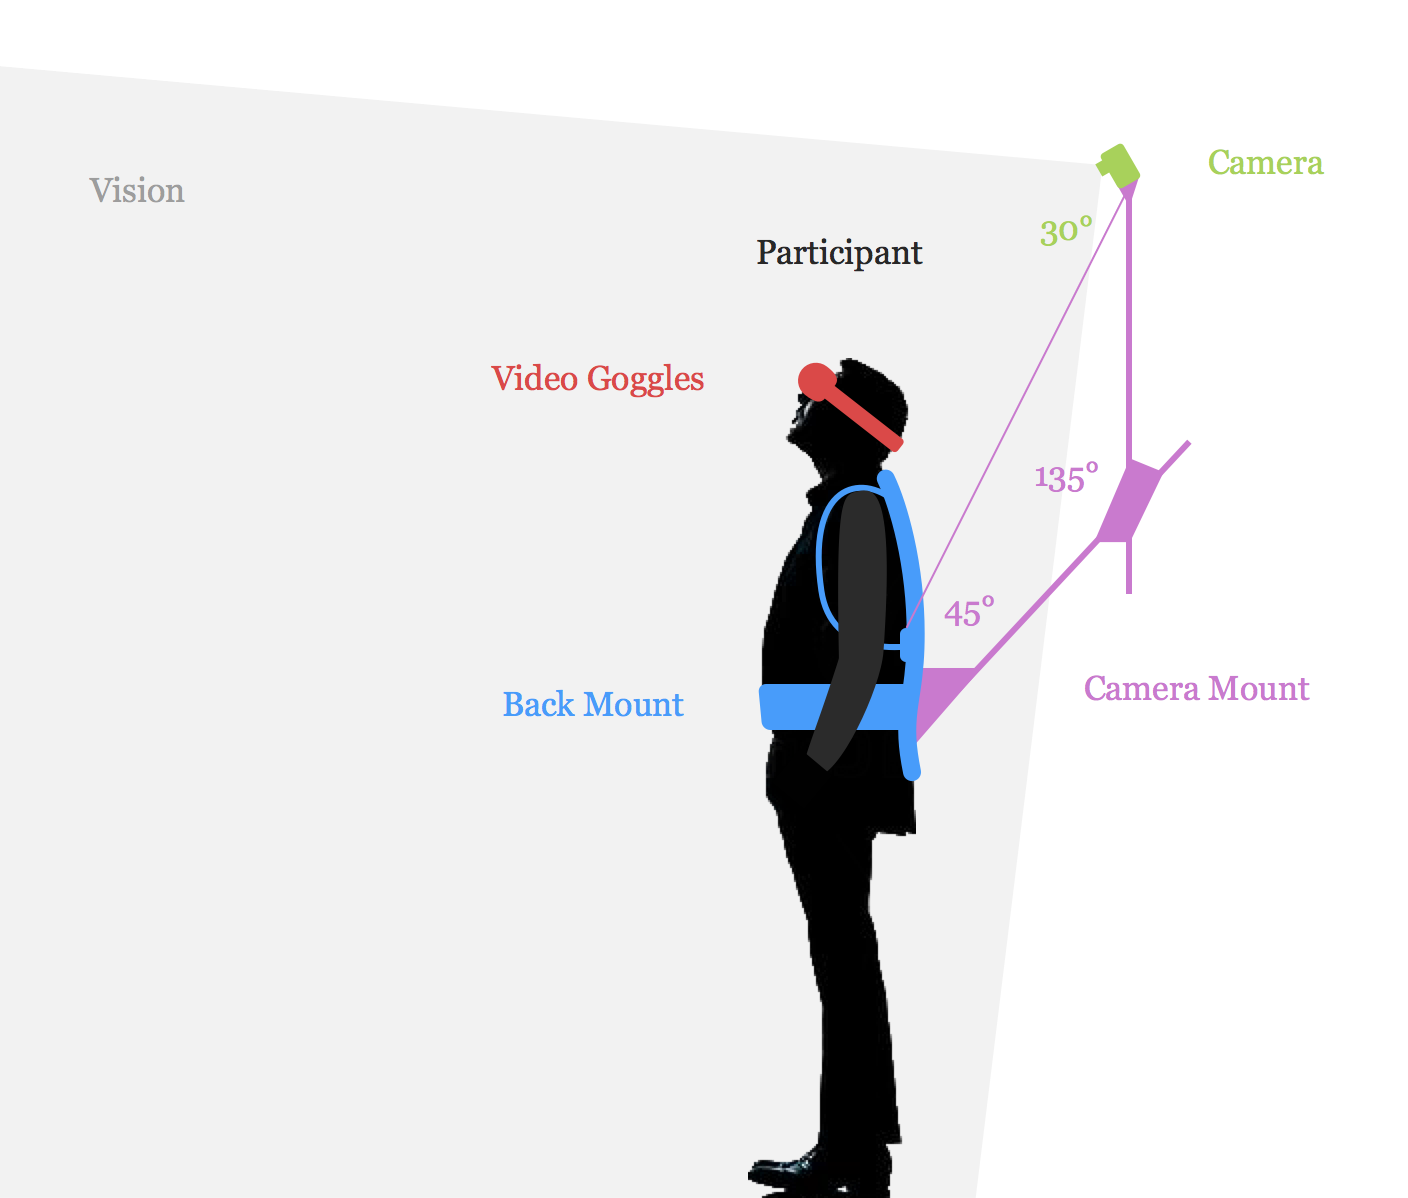
\includegraphics[width=0.8\textwidth]{ExternalMaterial/Rig}
   \caption{Illustration of different parts of the rig and how the fit together. \label{fig:RigDesign}}
\end{figure}








\subsection{Task Design} \label{subsec:TaskDesign}
Three different tasks were chosen to measure three separate areas; aiming accuracy, balance and movement control:

\subsubsection{Task 1: Accuracy}

The test subjects rolled, threw or bounced (depending on their preference) a multi-colored volleyball in order to try and hit a target (a regular sized chair) placed approximately 5 meters away to successfully complete the task. If the test subject missed the target they were told to try again until they finally hit it. This test measured the participants precise accuracy and ball control through the number of tries required in order to hit the target.

%\begin{figure}
%   \centering
%   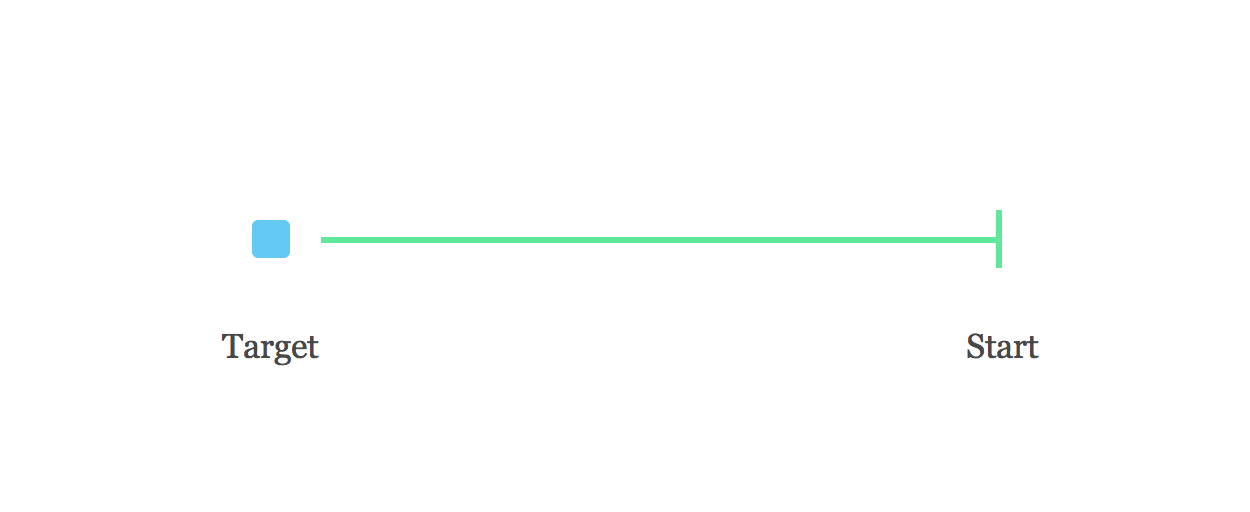
\includegraphics[width=0.7\textwidth]{ExternalMaterial/AccuracyTask}
%   \caption{A \emph{top-view} of the course used during Accuracy Task where green is tape on the floor and blue square is the chair.}. \label{fig:AccuracyTask}
%\end{figure}

\subsubsection{Task 2: Balance}

The test subjects walked in their preferred speed on a thin straight line made out of tape, 10 meters long placed on the ground. This test measured the participants balance skill through the number of errors they made. These errors were measured and recorded using one pre-defined rule; if any part of the shoe/foot covered at least the width of the tape (approximately 2 cm wide) it was considered to be a legal foot placement, everything else was illegal. Examples of illegal foot placements can be found in Figure \ref{fig:Illegal} and legal examples can be found in Figure \ref{fig:Legal}.


\begin{figure}
   \centering
   \includegraphics[width=0.6\textwidth]{ExternalMaterial/Illegal}
   \caption{Two examples of \textbf{illegal} foot placements.} \label{fig:Illegal}
\end{figure}
\begin{figure}
   \centering
   \includegraphics[width=0.6\textwidth]{ExternalMaterial/Legal}
   \caption{Two examples of \textbf{legal} foot placements.} \label{fig:Legal}
\end{figure}


%\begin{figure}
%   \centering
%   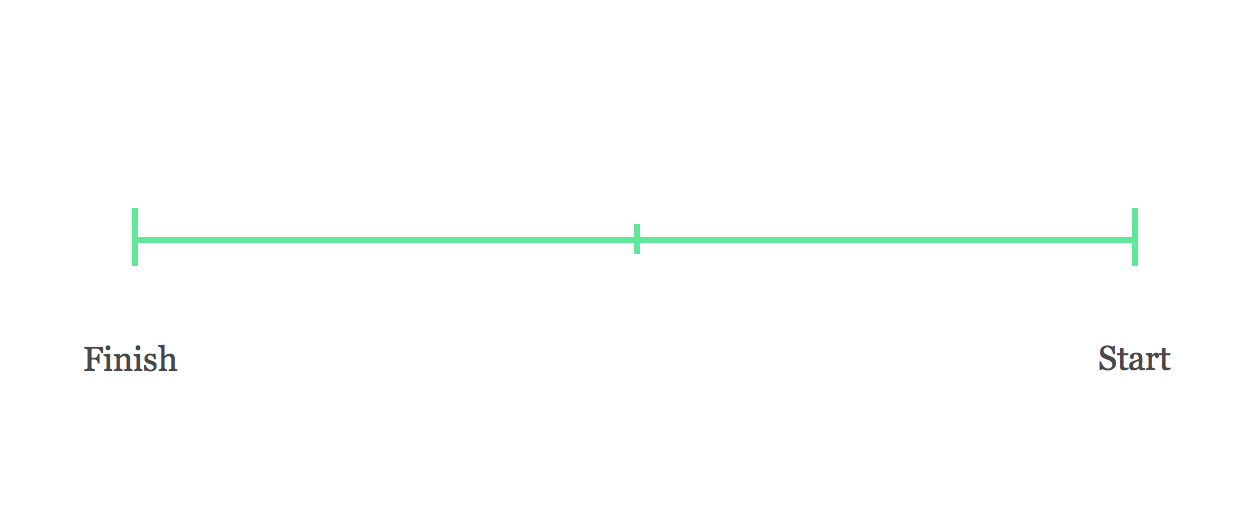
\includegraphics[width=0.7\textwidth]{ExternalMaterial/BalanceTask}
%   \caption{\emph{Top-view} of the course used during the Balance Task where green is tape on the floor.} \label{fig:BalanceTask}
%\end{figure}

\subsubsection{Task 3: Movement}

Test subjects walked facing forward in their normal walking speed, through a pre-planned course approximately 25 meters long and circa two\footnote{The actual width varied from around 1.5 to 2.5 meters throughout the course.} meters wide (see Figure \ref{fig:CourseTopSide}). Participants were told to do so without touching anything other than the floor. The course was constructed using 40 chairs, five tables, one large wooden box, a five meter long wall and a tall circular pillar. Participants started between two chairs and finished when they stepped on the cross marked with tape on the floor. This test measured the participants movement and navigational skills through the required time it took in order to complete the task. 
%Errors made, such as touching the chairs or tables, were also recorded.

%\begin{figure}
%   \centering
%   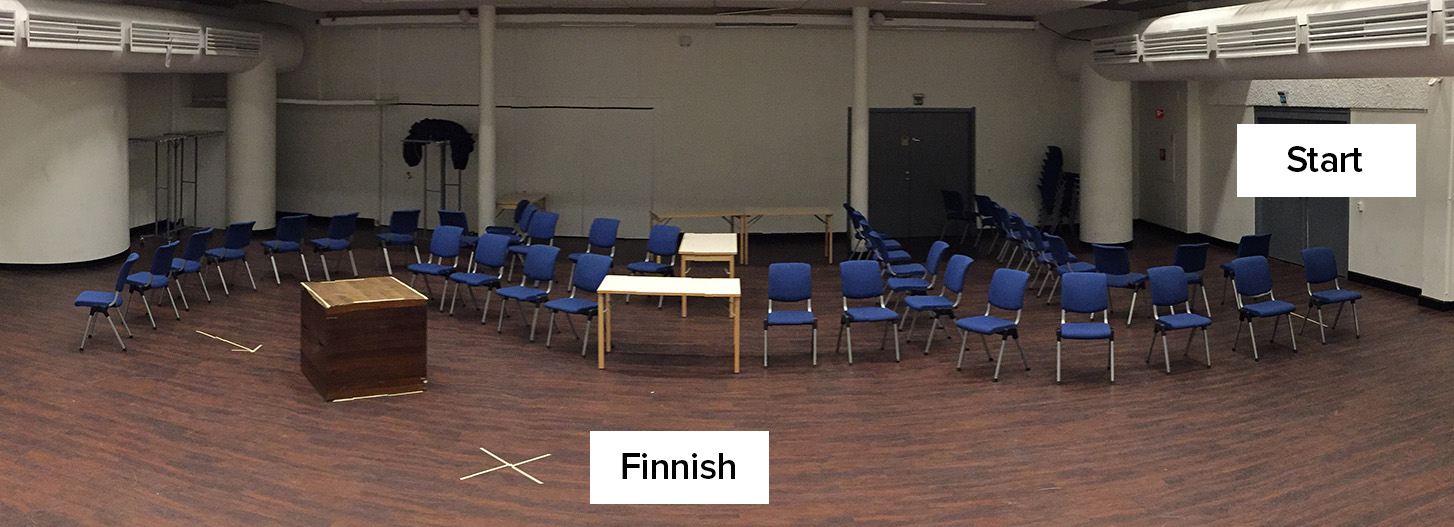
\includegraphics[width=\textwidth]{ExternalMaterial/Course2}
%   \caption{} \label{fig:Course}
%\end{figure}

\begin{figure}
   \centering
   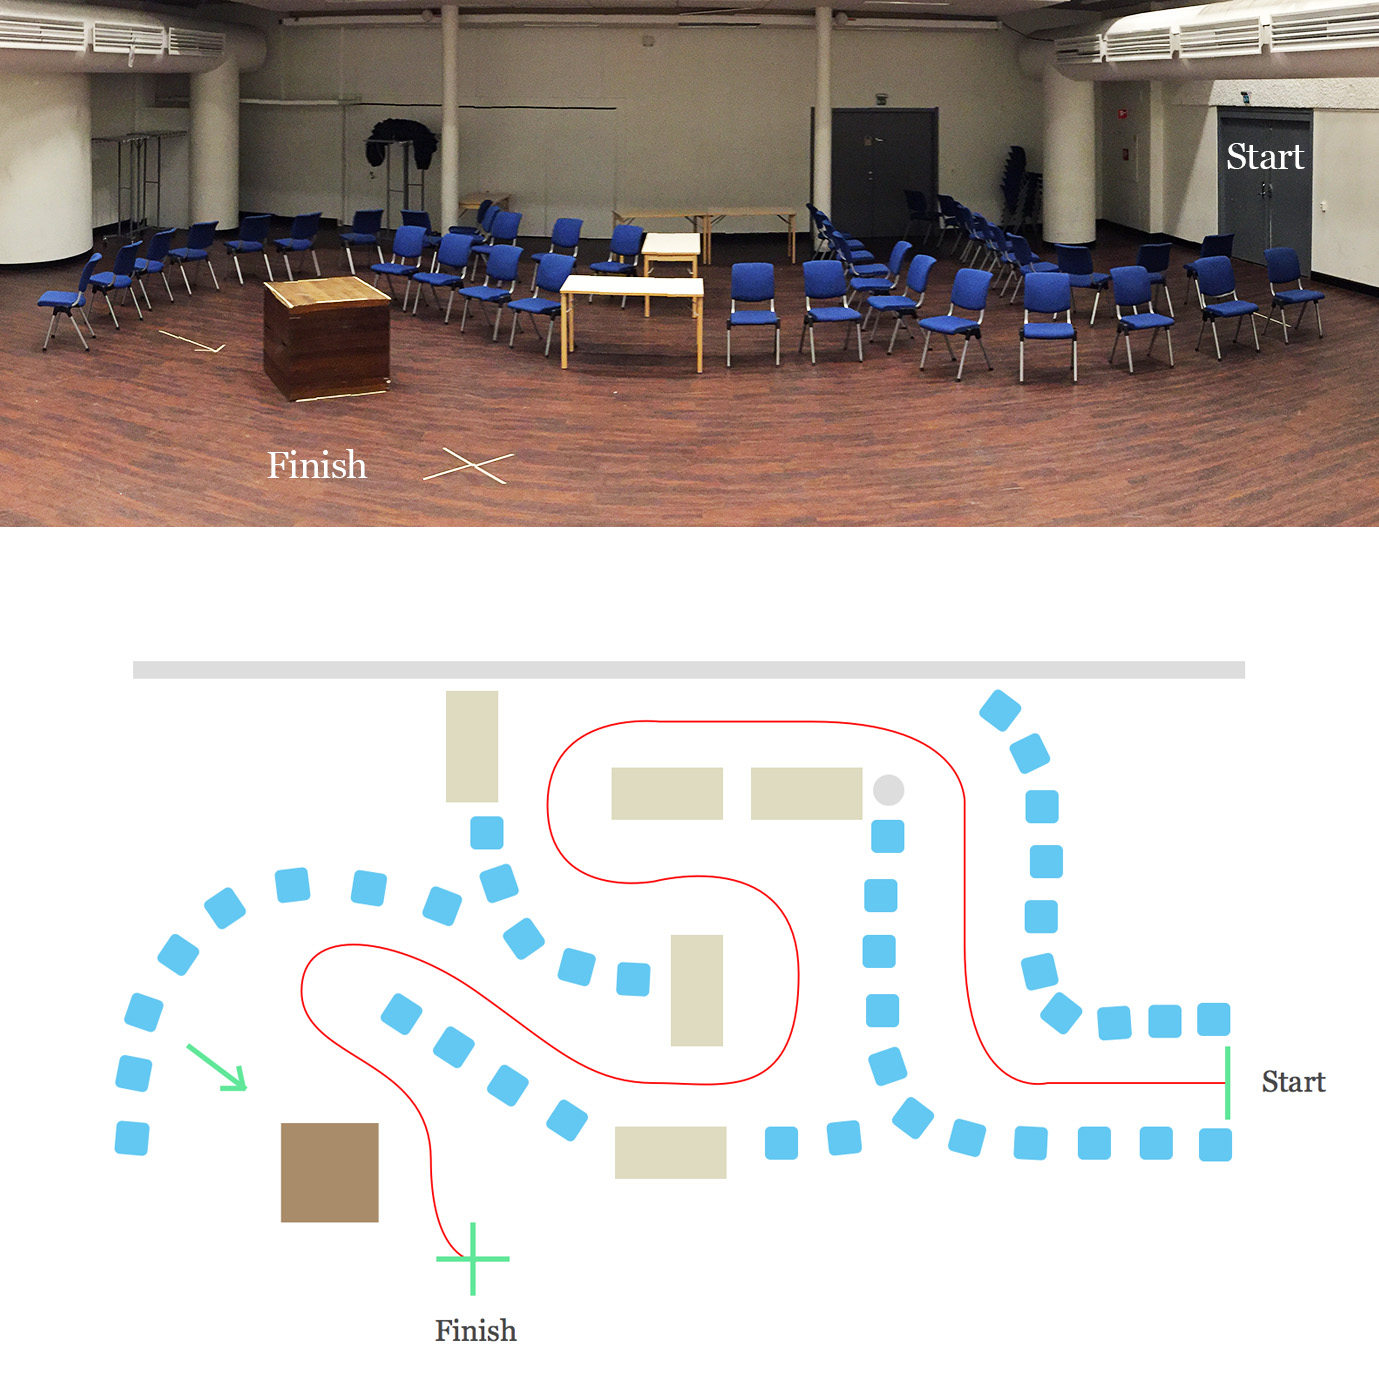
\includegraphics[width=\textwidth]{ExternalMaterial/Course-top-side}
   \caption{\textbf{At the top}: A \emph{side-view} of the course used during the Movement Task. \textbf{At the bottom}: A \emph{top-view} of the course used during the Movement Task. The thin, long red line is the approximate distance where the participants walked, the beige rectangles are tables, the small blue squares are chairs, the short green lines are tape on the floor, the large brown square is a wooden box, and the gray is the long wall and the circular pillar.} \label{fig:CourseTopSide}
\end{figure}








\subsection{Configurations} \label{subsubsec:Configurations}
Each task was performed three times by each participant, in three different configurations resulting in a total of nine results for each participant and task. The different configurations were completed in the following order:
\begin{enumerate}
	\item \textbf{Off}: \emph{Not} wearing the rig, video goggles \emph{off}.
	\item \textbf{First-Person}: Wearing the rig, video goggles \emph{on}, viewed from \emph{first-person} camera.
	\item \textbf{Third-Person}: Wearing the rig, video goggles \emph{on}, viewed from \emph{third-person} camera.
\end{enumerate} 

Completing the task three times was done to get a more accurate average of each of the participants performance. The first configuration served as a baseline for how a participant performs when completing the task ``normally''. The second configuration was used to compare against the first configuration in order to understand how much the video goggles and the first-person camera affected the participants performance in completing the tasks. Comparing the third and second configuration was the main focus of this study which was why the third configuration was the most critical one.















\subsection{Survey Design}
After each test subject finished his/hers participation in the experiment they were prompted to fill out a survey regarding the experience during the experiment and their prior experience with video games. The survey (the full form is found in the Appendix~\ref{subsec:Survey}) included the following seven questions:
\begin{enumerate}
	\item Do you consider yourself a \emph{gamer}?
	\item What was the hardest parts in the experiment?
	\item On average, how many hours per week do you spend playing video games?
	\item How many years have you been playing video games?
	\item In total, how many hours have you spent playing a game viewed from a third-person perspective?
	\item If any, please name some of these third-person games you have played.
	\item Did you find your participation in this experiment fun?
\end{enumerate}
Each test subject also filled in details about their name, age and sex so the results from the test data could be paired up with the surveys. The details were later removed in the results in order to keep the test subjects anonymity.

Questions 2 and 7 were asked in order to review the experiment, findings of which can be found in Section~\ref{subsec:AdditionalFindings}.




\subsection{Group Classification} \label{subsec:GroupClassification}
We classified each participant into one of the two groups, either the subject was a \emph{gamer} or a \emph{non-gamer}. While each subject had an opinion about which group they belonged in, the classification needed to be objective. In order to be regarded as a gamer the subject had to fulfill four requirements:
\begin{enumerate}
   \item An average of five hours or more spent playing games every week. 
   \item A total of more than 80 hours playtime in a third-person game.
   \item Seven years or more of experience playing video games.
   \item Listing at least three third-person games they have played.
\end{enumerate}


%


%From the results in the survey six participants classified themselves as gamers while the rest as non-gamers.






















% 8888888b.  8888888888 .d8888b.  888     888 888    88888888888 
% 888   Y88b 888       d88P  Y88b 888     888 888        888     
% 888    888 888       Y88b.      888     888 888        888     
% 888   d88P 8888888    "Y888b.   888     888 888        888     
% 8888888P"  888           "Y88b. 888     888 888        888     
% 888 T88b   888             "888 888     888 888        888     
% 888  T88b  888       Y88b  d88P Y88b. .d88P 888        888     
% 888   T88b 8888888888 "Y8888P"   "Y88888P"  88888888   888

\section{Results}
The statistical tests used in the results are paired, two tailed t-tests.

%\subsection{Task Performance}
%The following are results when comparing the two groups, gamers and non-gamers, in each of the executed tasks in the experiment.


\subsubsection{Accuracy Task}
As seen in Table~\ref{tab:Task1GraphP} the average performance, as in number of tries required in order to hit the target, is generally good (as in a low number of tries) for both groups. Whilst the average gamer\footnote{The average of the results from all the gamers.} generally performed slightly better in both first- and third-person configurations, there is no significant difference (p-value at 0.63) between the two groups.

Furthermore, looking at the graph in Figure \ref{fig:Task1GraphD} we see that the percental average individual difference in performance is generally lower for gamers. This indicates that the average gamer had less trouble with readjustment when changing between the different configurations. This conclusion could however not be statistically confirmed (p-value at 0.54).


\begin{table}[]
\centering

\setlength{\tabcolsep}{1em}
%\setlength\extrarowheight{0.8em}
\def\arraystretch{1.8}
\begin{tabular}{l|c|cll}
                      & {\textbf{Gamers}} & {\textbf{Non-gamers}} &  &  \\ \cline{1-3}
\textbf{1. Off}          & 1.3 tries                                   & 1 tries                                          &  &  \\ \cline{1-3}
\textbf{2. First-Person} & 1.5 tries                                    & 1.6 tries                                        &  &  \\ \cline{1-3}
\textbf{3. Third-Person} & 1.7 tries                                    & 1.9 tries                                        &  & 
\end{tabular}
\caption{Average performance (tries required before hitting the target, where less is better) for the two groups for the Accuracy Task for the three test configurations. Standard deviation stretching from 0.2 (non-gamers in configuration one) to 1.2 (gamers in configuration three) at most.}
\label{tab:Task1GraphP}
\end{table}




%\begin{figure}
%   \centering
%   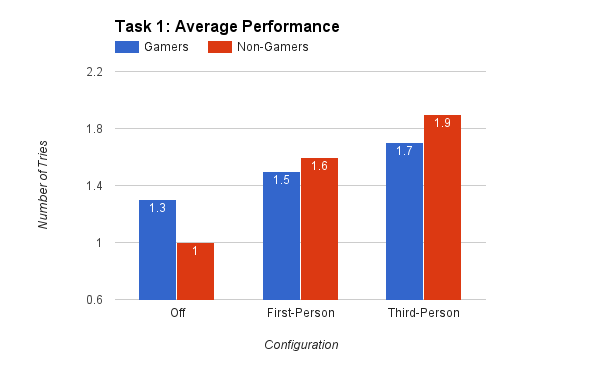
\includegraphics[width=\textwidth]{ExternalMaterial/Task1GraphP}
%   \caption{Average performance (tries required, less is better) for the two groups for task 1, rounded to one decimal place.} \label{fig:Task1GraphP}
%\end{figure}

\begin{figure}
   \centering
   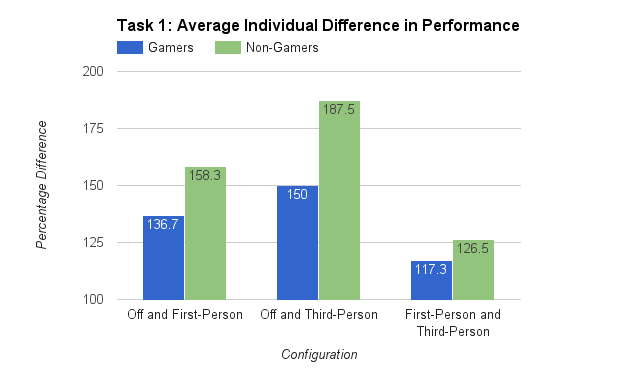
\includegraphics[width=\textwidth]{ExternalMaterial/Task1GraphD}
   \caption{Average individual difference (percent, less is better) in performance (tries required, less is better) between two configurations for the two groups for the accuracy task. Standard deviation stretching from 49.2 (non-gamers comparing configuration two and three) to 81.5 (non-gamers comparing configuration one and two). For example, the average individual throws required for a gamer in configuration three is 150\% of the required throws in configuration one, therefor 50\% worse/more.} \label{fig:Task1GraphD}
\end{figure}











%Noteworthy is also the fact that none of the participants, in any of the groups, made any illegal foot placements during the first configuration (not wearing any equipment) suggesting that the task might have been too straightforward.

\subsubsection{Balance Task}
Unlike the results from the accuracy task, on an average, a gamer performed slightly \emph{worse} than a non-gamer in the third-person configuration. As seen in Table~\ref{tab:Task2GraphP} the only notable difference between the groups is the last configuration. The numbers of illegal steps dramatically increased when viewed from third-person view, from 0 (for both groups) to 9.7 (non-gamers) respectively 12.3 (gamers) steps.  

When turning our attention towards the percental average individual difference in performance presented in Figure \ref{fig:Task2GraphD} we could only conclude that the average gamer had less difficulty with readjustment when changing between the last two configurations\footnote{Although the standard deviation was generally high at 528 amongst non-gamers, respectively 160 between gamers.}. This hypothesis was rejected after a t-test (p-value at 0.59).


\begin{table}[]
\centering
\setlength{\tabcolsep}{1em}
%\setlength\extrarowheight{0.8em}
\def\arraystretch{1.8}
\begin{tabular}{l|c|cll}
                      & {\textbf{Gamers}} & {\textbf{Non-gamers}} &  &  \\ \cline{1-3}
\textbf{1. Off}          & 0 errors                                    & 0 errors                                          &  &  \\ \cline{1-3}
\textbf{2. First-Person} & 4.3 errors                                   & 4.5 errors                                        &  &  \\ \cline{1-3}
\textbf{3. Third-Person} & 12.3 errors                                    & 9.7 errors                                        &  & 
\end{tabular}
\caption{Average performance (errors made while walking the line, where less is better) for the two groups for the balance task. Standard deviation first-person configuration was 2 for gamers and 3.7 for non-gamers, respectively 3.4 and 4.4 for third-person configuration. No deviation for the first configuration for any of the groups.}
\label{tab:Task2GraphP}
\end{table}




%\begin{figure}
%   \centering
%   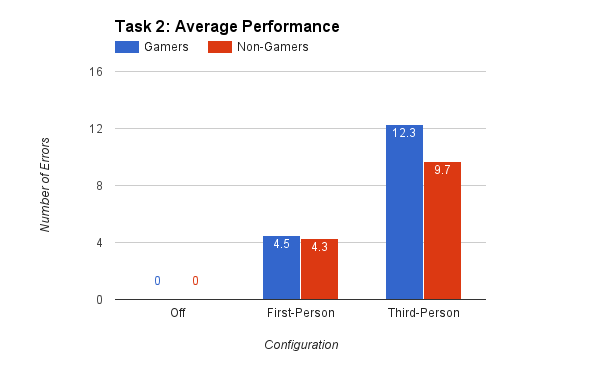
\includegraphics[width=\textwidth]{ExternalMaterial/Task2GraphP}
%   \caption{Average performance (errors made, less is better) for the two groups for task 2.} \label{fig:Task2GraphP}
%\end{figure}

\begin{figure}
   \centering
   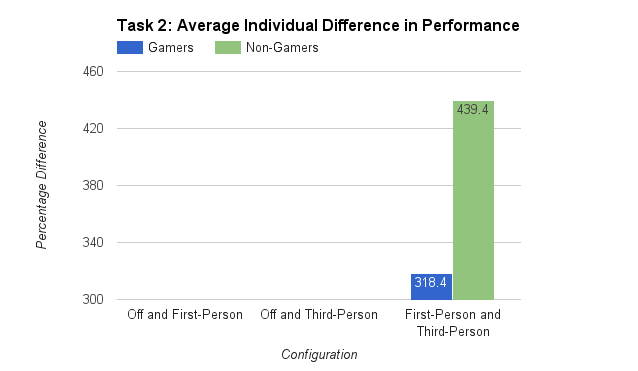
\includegraphics[width=\textwidth]{ExternalMaterial/Task2GraphD}
   \caption{Average individual difference (percent, less is better) in performance (errors made while walking the line, less is better) between the second and third configurations for the two groups for the balance task. For example, the average individual number of errors for a gamer in configuration three is 318.4\% of the number of errors in configuration two, therefor 218.4\% worse/more. The first two comparisons (first and second configuration, first and third configuration) were inconclusive due to the first configuration being 0 for both groups, therefore not comparable.} \label{fig:Task2GraphD}
\end{figure}











\subsubsection{Movement Task}
Similarly to the findings in the balance task, results in the movement task (found in Table~\ref{tab:Task3GraphP}) suggest that the average gamer performs worse, as in more time required to complete the course, than the average non-gamer. 

%Whilst average performance among the two groups is interesting, it is irrelevant for this task in particular. This might be due to the individual differences, such as having a lower normal walking speed or being more cautious when completing the course. 
Turning our attention towards Figure \ref{fig:Task3GraphD} we can see that the percental average individual difference in performance is generally higher (0.2, 4, and 6.7 seconds) for the average gamer than the average non-gamer. Unlike in the two earlier tasks this result was confirmed (p-value at 0.02), after establishing that both datasets are normally distributed with a normality test.

%While this might look like a significant find, it is hard to prove that this is not due to pure luck induced by the rather low number of participants in the study.





\begin{table}[]
\centering
\setlength{\tabcolsep}{1em}
%\setlength\extrarowheight{0.8em}
\def\arraystretch{1.8}
\begin{tabular}{l|c|cll}
                      & {\textbf{Gamers}} & {\textbf{Non-gamers}} &  &  \\ \cline{1-3}
\textbf{1. Off}          & 20.9 seconds                                    & 20.7 seconds                                          &  &  \\ \cline{1-3}
\textbf{2. First-Person} & 33 seconds                                   & 29.6 seconds                                        &  &  \\ \cline{1-3}
\textbf{3. Third-Person} & 40.7 seconds                                    & 34 seconds                                        &  & 
\end{tabular}
\caption{Average performance (time required in order to finish the course, where less is better) for the two groups for the movement task.}
\label{tab:Task3GraphP}
\end{table}

%SKRIVA OM STANDARDAVVIKELSE


%\begin{figure}
%   \centering
%   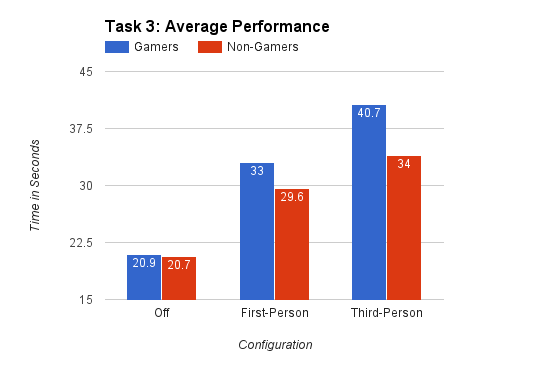
\includegraphics[width=\textwidth]{ExternalMaterial/Task3GraphP}
%   \caption{Average performance (time required, less is better) for the two groups for task 3.} \label{fig:Task3GraphP}
%\end{figure}

\begin{figure}
   \centering
   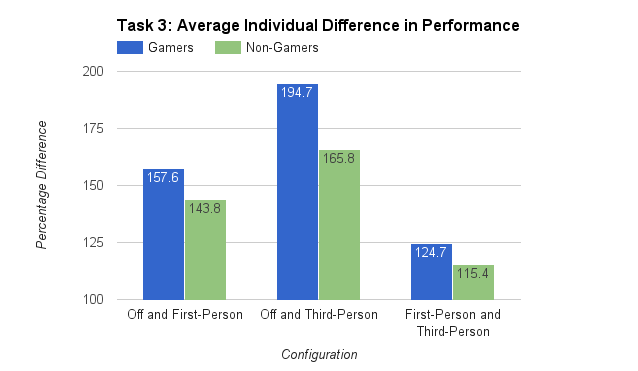
\includegraphics[width=\textwidth]{ExternalMaterial/Task3GraphD}
   \caption{Average individual difference (percent, where less is better) in performance (time required in order to finish the course, where less is better) between two configurations for the two groups for the movement task. For example, the average individual time required for a gamer in configuration two is 157.6\% of the time required in configuration two, therefor 57.6\% worse/more.} \label{fig:Task3GraphD}
\end{figure}























% 8888888b. 8888888 .d8888b.   .d8888b.  888     888  .d8888b.   .d8888b.  
% 888  "Y88b  888  d88P  Y88b d88P  Y88b 888     888 d88P  Y88b d88P  Y88b 
% 888    888  888  Y88b.      888    888 888     888 Y88b.      Y88b.      
% 888    888  888   "Y888b.   888        888     888  "Y888b.    "Y888b.   
% 888    888  888      "Y88b. 888        888     888     "Y88b.     "Y88b. 
% 888    888  888        "888 888    888 888     888       "888       "888 
% 888  .d88P  888  Y88b  d88P Y88b  d88P Y88b. .d88P Y88b  d88P Y88b  d88P 
% 8888888P" 8888888 "Y8888P"   "Y8888P"   "Y88888P"   "Y8888P"   "Y8888P"  

\section{Discussion} \label{sec:Discussion}
Earlier work suggest that third-person perspective causes no significant discomfort while at the same time having a short learning time~\cite{nakamura20103pi}, something we found contradictory to our results. Participants generally performed worse when executing all tasks in the second configuration (first-person perspective) compared to the first (normal viewing) configuration. Subjects normally performed even worse in the third-person configuration, somewhat rejecting earlier findings. 


\subsection{Additional Findings} \label{subsec:AdditionalFindings}
Since the low amount of participants in the study influence the results, no final conclusions can be made about the difference in performance between third-person view and normal viewing when comparing gamers and non-gamers. However, additional findings where made during the experiments, these include:
\begin{itemize}
	\item All 13 participants in the study said they found the third-person view (configuration three) difficult while only five did for the second configuration (first-person view).

	\item Walking on a straight line on the floor (as participants did in the balance task) in third-person view (configuration three) was exceptionally hard regardless to the subjects gaming background and sex. This was due to the lack of vision of the line in front of the participants feet and body while walking. 

	\item What defines a \emph{gamer} is more of a subjective opinion than an objective classification. This became apparent when using the objective group classification (described in Section~\ref{subsec:GroupClassification}), five subjects, where four considered themselves as gamers, meet the criteria. However two participants, that both considered themselves as gamers, did not meet the criteria and where therefore referred to as non-gamers.

	\item Familiarizing participants with the concept of moving their field of view using their hips rather than their neck turned out to require more time than first anticipated. Even after 15 minutes of wearing the rig in third-person perspective participants were moving their neck instead of their hips to look around.

	\item Depth perception is generally hard when viewing a camera stream from a wide field of view camera lens, especially without stereoscopic vision.

	\item Although most participants felt slightly nauseated after the experiment, none lost complete balance and fell. As a plus, all participants said they enjoyed taking part in the experience.

   \item Findings amongst non-gamers suggest that there is no significant measurable difference in performance between the sexes for any of the tasks in any configuration.
\end{itemize}





\subsection{Limitations and Drawbacks}
Due to the time and budget limitations there are several ways to improve upon our experiments. The largest, and possibly most significant, is the low number of participants in the study. Other limitations and drawbacks include:
\begin{description}
	\item[Rig Design] Although the rig was rigid enough for this particular experiment, reinforcements should be made in order to continue with further testing. The biggest drawback of the current rig are the shakes generated on fast movements such as running or fast turns. This could be fixed by connecting one, or preferably two, more booms on an angle to both the back mount and the current booms to counteract horizontal and vertical vibrations. Another solution could also be to purchase an already tested and viable rig such as the \emph{3rdPersonView}\footnote{More info can be found at http://www.sailvideosystem.com/p/3rdpersonview-all-sports-pro-166682} from \emph{Sail Video System}.

	\item[Camera Movement] Normally in a virtual third-person game, such as GTA (see Figure \ref{fig:GTAIV}), the ``camera'' follows the characters movements with a slight delay in order to get more fluid camera movements. The current setup does not currently support this due to the cameras fixed attachment to the back mount, however this could be corrected using a three-axis gimbal, something that would also improve the overall stability of the camera. Adding an IMU\footnote{Inertial Measurement Unit, such as a gyroscope and an accelerometer} to the users video goggles would also allow for the user to look around using his/hers normal head movements.

	\item[Task Design] The tests chosen for this study, especially the task one and two, aimed to test specific abilities, such as accuracy, balance and navigation. While this is a start, more relevant and less specific test could be conducted using more everyday-like tasks, such as riding a bike, walking to work, cooking food etc.

	\item[Video Goggles] Whilst the video goggles used had an average resolution, more sophisticated video goggles, such as the \emph{Oculus Rift}\footnote{More info can be found at https://www.oculus.com/en-us/rift/} or the \emph{HTC Vive}\footnote{More info can be found at http://www.htcvr.com/}, with a higher pixel count could be used to create a more immerse and believable simulation. Since both of these are made for virtual reality gaming, their field of view is notably greater than in the \emph{SkyZone} goggles used. Using an actual VR headset would also add stereoscopic vision, a feature that might have made a difference on our results.

	\item[More Segregated Groups] As discussed earlier in Section~\ref{sec:Discussion}, the definition of \emph{what defines a gamer} is not apparent. Since none of the student volunteers were professional, full-time gamers we cannot make any statements about \emph{actual gamers}\footnote{A person who spends most of their awake time playing games, mostly professionally but also casually}. The same goes for non-gamers; most of our subjects have sometime in their life been exposed to video games to some extent, either playing themselves or watching someone else playing. This results in oblique findings about non-gamers as well.

	\item[Sex Ratio] Due to the high male skew in the study (especially amongst gamers), no conclusive findings about difference, or indifference, between males and females were found.
\end{description}



\subsection{Conclusion}
We believe this study should serve as a foundation and a guide for further research in the future and not as reference material for any hard proof. In order to fully study the differences between the groups one would need a larger participant group with a greater segregation in time spent playing video games.









%        d8888  .d8888b.  888    d8P  888b    888  .d88888b.  888       888 
%       d88888 d88P  Y88b 888   d8P   8888b   888 d88P" "Y88b 888   o   888 
%      d88P888 888    888 888  d8P    88888b  888 888     888 888  d8b  888 
%     d88P 888 888        888d88K     888Y88b 888 888     888 888 d888b 888 
%    d88P  888 888        8888888b    888 Y88b888 888     888 888d88888b888 
%   d88P   888 888    888 888  Y88b   888  Y88888 888     888 88888P Y88888 
%  d8888888888 Y88b  d88P 888   Y88b  888   Y8888 Y88b. .d88P 8888P   Y8888 
% d88P     888  "Y8888P"  888    Y88b 888    Y888  "Y88888P"  888P     Y888 

\section{Acknowledgments}
The authors would like to thank all participants in the study for their time, participation and feedback. We would also like to thank all the peer-reviewers (especially \emph{Lars Englund} for his help during the experiments) who helped form this report into its final shape along with \emph{David Källberg} for his help with the statistical analysis of the data. Last but not least we would like to thank \emph{Umeå University} for letting us use their facilities \emph{Rotundan} (where we conducted our experiments) and \emph{Robotlabbet} (where we constructed the rig) during the progress of the study.







%\nocite{*}
\bibliographystyle{splncs}
%\bibliographystyle{plain-annote}

\bibliography{Bibliography}

\appendix

\section{Appendix}
All the files for this report, along with all the 3D-design-files and experiment results can be found and downloaded on the GitHub-page\footnote{More info can be found at https://github.com/Kodagrux/Third-Person-Performance-Differences-Between-Gamers-and-Nongamers} for this project.
\subsection{Survey} \label{subsec:Survey}
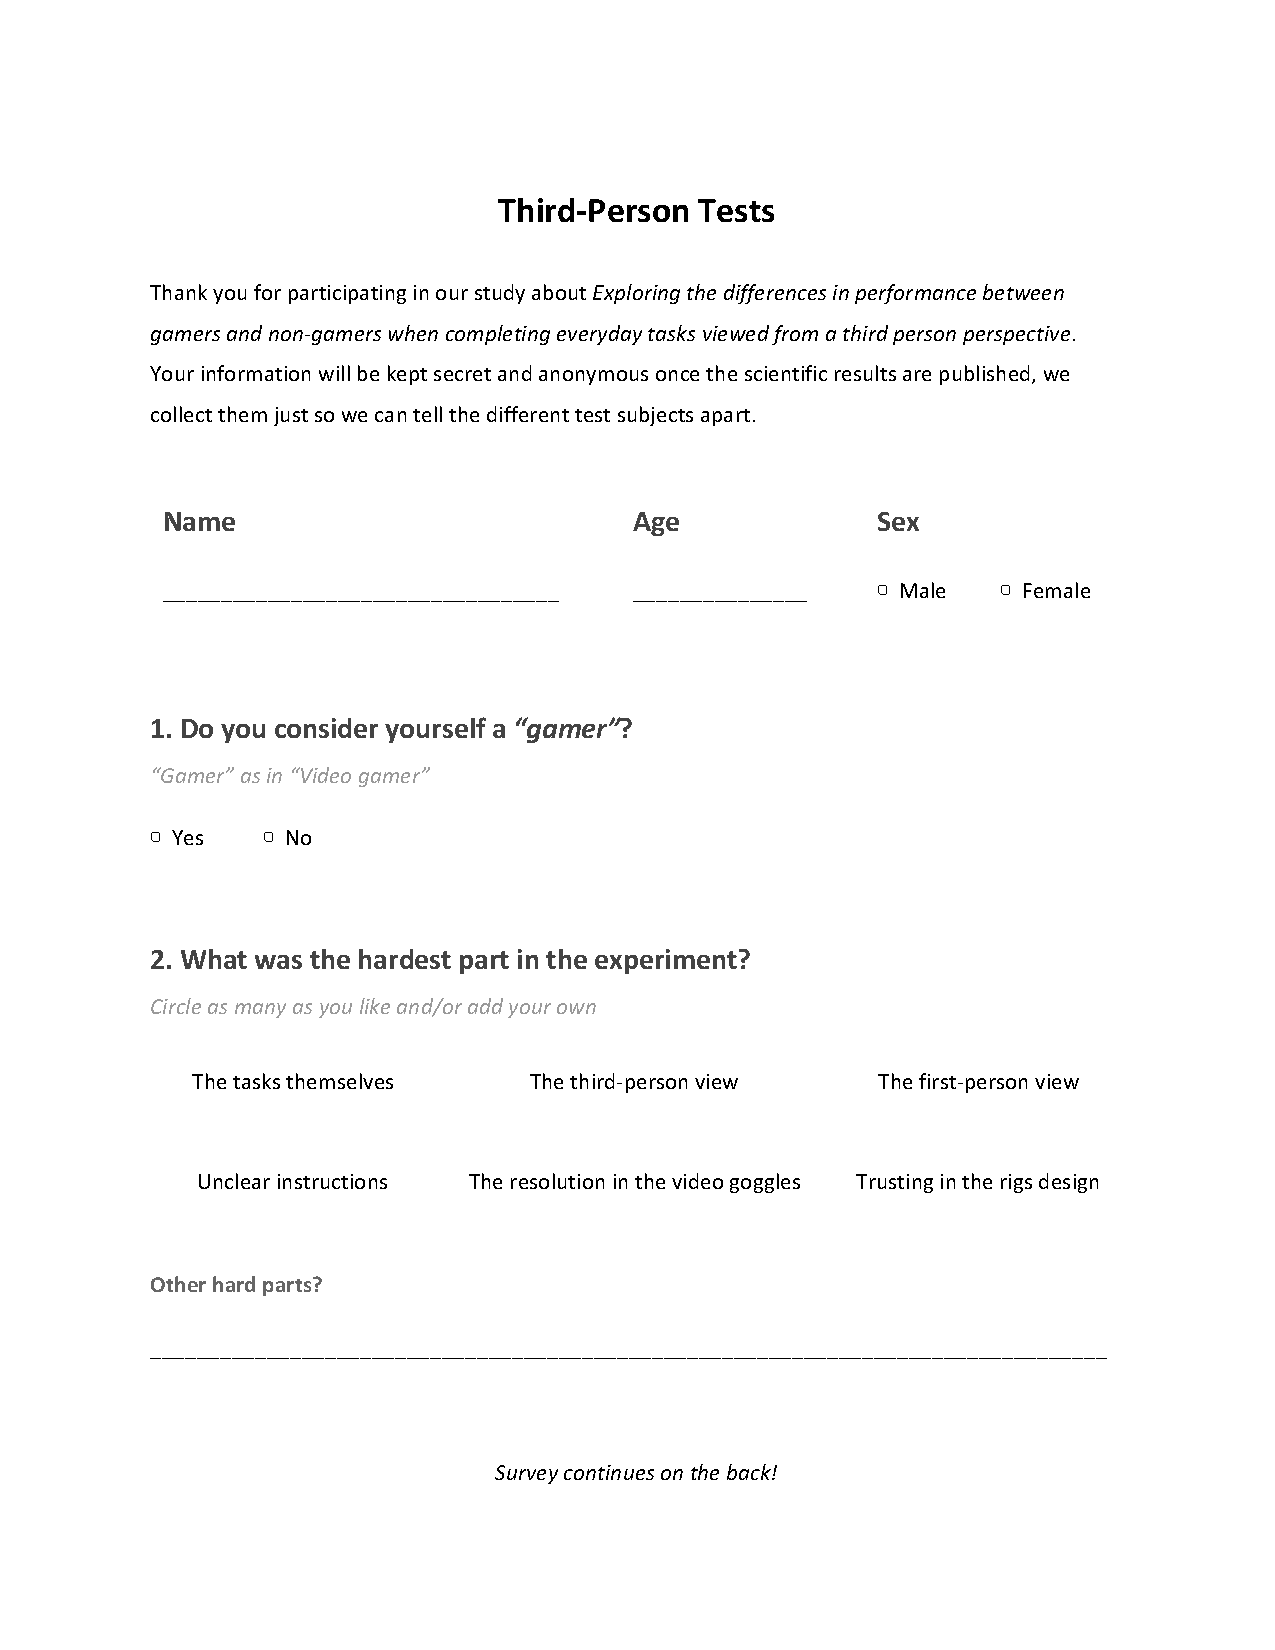
\includepdf[pages={1-2}]{ExternalMaterial/Survey.pdf}


\end{document}